\documentclass[12pt,a4]{article}

\usepackage[utf8]{inputenc}
\usepackage[T1]{fontenc}
\usepackage{amsmath,amsfonts}
\usepackage{graphicx}
\usepackage{enumerate}
\DeclareMathOperator*{\argmin}{\arg\!\min}

\newcommand{\R}{{\mathbb R}}
\newcommand{\C}{{\mathbb C}}
\newcommand{\N}{{\mathbb N}}
\newcommand{\ra}{\rightarrow}
\newcommand{\lra}{\longrightarrow}
\newcommand{\lnorm}{\left\|}
\newcommand{\rnorm}{\right\|}
\newcommand{\ind}{{\mathbf{1}}}

\newcommand{\citeneeded}{\ensuremath{\vphantom{1}^{\text{[citation needed]}}\,}}
\newcommand{\eps}{\ensuremath{\varepsilon}}


\title{Glottal inversion with an approximate vocal tract filter}
\author{Lasse Lybeck, Robert Sirviö}


\begin{document}

\maketitle

%---------------------Introduction--------------------
\section{Introduction}\label{sec:intro}

A synthetic human vowel sound consists of a periodic signal to simulate the glottal excitation signal at the glottis and a filter to simulate the vocal tract, which the glottal signal is filtered through.\citeneeded With a given vocal tract filter the direct problem is \emph{given a glottal excitation signal, create the vowel sound}. The inverse problem is \emph{given a (recorded) vowel sound, find the glottal excitation signal}. In this study we will be concentrating on the inverse problem, starting with both a simulated vowel and a real recording.

The inversion from a vowel sound to the glottal signal is an important part of creating synthetic human voices and speech generators. To create a synthetic vowel both the glottal signal and the vocal tract filter are needed. However, the glottal signal cannot be directly measured, but it can be approximated with inversion of a recorded vowel. With this data models for simulating the glottal excitation signal can be created.


%-----------------Materials & Methods-----------------
\section{Materials and Methods}\label{sec:methods}

\subsection{Glottal excitation signal}
\label{sec:rk}

In this study the Rosenberg-Klatt model (RK-model) for the glottal excitation signal will be used for the generation of synthetic data and as a reference point for the obtained results. The RK-model is a simple model for the glottal signal, proposed in 1970 by Rosenberg.\cite{rosenberg} The model is simple and easy to use, as it creates the signal only from two parameters, the sound frequency $f$ and the so called Klatt-parameter $Q$.

The \emph{airflow} for the glottal excitation signal created by the RK-model is defined as
\begin{equation}
\label{eq:RK-model}
g(t) =
  \begin{cases}
   at^2 + bt^3  & \text{jos } 0 \leq t \leq Q T \\
   0            & \text{jos } Q T < t \leq T,
  \end{cases}
\end{equation}
where $t$ is a time variable, $T = 1/f$ is the period of the pitch, $Q \in \left[ 0,1 \right]$ is the Klatt-parameter and $a$ and $b$ are variables defined in terms of $T_0 := QT$ as
\begin{equation*}
a = \frac{27}{4 T_0^2}, \quad b = -\frac{27}{4 T_0^3} .
\end{equation*}
Here the parameter $f$ defines the frequency of the generated signal and the Klatt-parameter $Q$ defines the shape of the pulse.

The glottal excitation signal can be retrieved as the derivative $g'$ of the airflow function. Here $g'$ is the \emph{pressure function}, and simulates the sound generated in the glottis. The pulse generated by the model can be seen in figure \ref{fig:klatt}.

Another, more widely used, model for the glottal excitation signal worth mentioning is the Liljencrants-Fant model (LF-model).\cite{fant} It is regarded as more accurate than the RK-model, but it is also much more complex. It has also been shown, that the LF-model generates only marginally better approximations for the resulting vowel after the vocal tract filtering than the RK-model.\cite{fujisaki} Due to this and the overall complexity of the LF-model we will be using the RK-model for the simulation of the glottal exitation signal in this study.

\begin{figure}[t]
\begin{center}
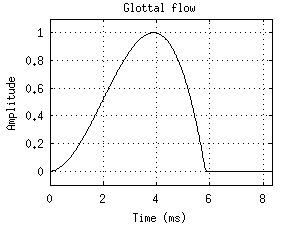
\includegraphics[scale=1]{img/klattflow.png}
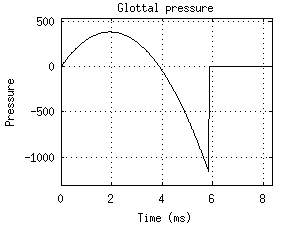
\includegraphics[scale=1]{img/klattpres.png}
\end{center}
\caption{The airflow and pressure generated by the RK-model}
\label{fig:klatt}
\end{figure}


\subsection{Vocal tract filter}
\label{sec:filter}

In this study we will assume an approximate vocal tract filter to be known for the recorded vowel we want to invert. The digital filter, defined by a vector $a \in \R^{N_a}$, filters the data $x \in \R^n$ as defined by the difference equation
\begin{equation}
\left\{
\begin{alignedat}{1}
\label{eq:filter-diffeq}
y_1     &= x_1 \\
a_1 y_j &= -\sum_{k=2}^{\min\{j-1, N_a\}} a_{k} y_{j-k} ,
\end{alignedat}
\right.
\end{equation}
where $y \in \R^n$ is the filtered data. We denote $y = \varphi_a (x)$.

Consider now the filter defined by $a \in \R^{N_a}$ and the data $x \in \R_n$ which we want to filter. Now the filter defined by \eqref{eq:filter-diffeq} can be expressed by the the matrix $A \in \R^{n \times n}$, where
\begin{equation}
\left\{
\begin{alignedat}{3}
   &A_{1,1}     = a_1 \\
   &A_{i,1}     = - \sum_{k=1}^{\min\{ i-1, N_a-1 \}} a_{k+1} A_{i-k,1}, \quad && 2 \leq i \leq n \\
   &A_{i+1,j+1} = A_{i,j},     && j \leq i \\
   &A_{i,j}     = 0,           && j > i .
\end{alignedat}
\right.
\end{equation}
Now $\varphi_a (x) = Ax$.


\subsection{The matrix model}
\label{sec:matrixModel}

A vowel sound can be simulated by applying a digital filter $A\in\R^{n \times n}$ to a sample of a glottal excitation signal $f \in \R^n$ as
\begin{equation}
\label{eq:vow}
v = A f,
\end{equation}
where $v \in \R^n$ is the simulated vowel. In this study we will assume an approximation of the filter $A$ to be known. Given the measurement $m \in \R^n$ of a vowel corresponding approximately to the filter $A$, equation \eqref{eq:vow} can be expressed as
\begin{equation}
\label{eq:vowModel}
m = A f + \eps,
\end{equation}
where $\eps \in \R^n$ denotes the measurement noise.


\subsection{The inversion method}\label{sec:invMethod}

\subsubsection{Tikhonov reguralization}\label{sec:tikh}
The classical Tikhonov regularized solution for $m = Ag + \varepsilon$, defined in section \ref{sec:matrixModel}, is usually denoted by the vector $T_\alpha(m)\in\R^n$ that minimizes
\begin{equation*}
\lnorm AT_\alpha(m) - m \rnorm^2 + \alpha \lnorm T_\alpha(m) \rnorm^2 \Leftrightarrow
\end{equation*}
\begin{equation*}
T_\alpha(m) = \underset{z\in\R^n}{\argmin}
\left\{ \lnorm Az - m \rnorm^2 + \alpha \lnorm z \rnorm^2 \right\},
\end{equation*}
where $\alpha > 0$ is called a regularization parameter. The resulting $T_\alpha(m)$ can be understood as a compromise between two conditions, namely
\begin{enumerate}[I.]
 \item $T_\alpha(m)$ should give a small residual $AT_\alpha(m) - m$.
 \item $\lnorm T_\alpha(m) \rnorm_2$ should be small.
\end{enumerate}
The $\alpha$ parameter is used in order to tune to balance between the two conditions above.

In generalized Tikhonov regularization some prior knowledge is assumed to be known. In some cases $g$ might be known to be smooth. This information can be incorporated into the regularization by choosing
\begin{equation}
T_\alpha(m) = \underset{z\in\R^n}{\argmin}
\left\{ \lnorm Az - m \rnorm^2 + \alpha \lnorm Lz \rnorm^2 \right\},
\end{equation}  
where $L$ is a discretized differential operator.
 
In our model proposed in section \ref{sec:rk} we know the airflow of the excitation signal to be smooth in the interval $[0, QT]$ and to be zero in the interval $]QT, T]$. This can be incorporated in our model by customizing the discrete differential operator matrix, described in more detail in section \ref{sec:basis}


\subsubsection{The conjugate gradient method}\label{sec:conjgrad}


\subsubsection{Morozov's discrepancy principle}
The problem of finding the optimal regularization parameter is, in general, considered to be unsolved. There are, however, methods that attempt to find an optimal choice of the regularization parameter, including the Mozorov discrepancy principle, which is based on the noise level in the data.

Assume that we know the size of the noise in our model defined by \eqref{eq:vowModel} to be $\delta > 0$. Now $T_\alpha(m)$ is an acceptable reconstruction if 
\begin{equation}
\lnorm AT_\alpha(m)-m\rnorm \leq \delta
\end{equation}

\subsection{The basis and materials}\label{sec:basis}
%-----------------------Results-----------------------
\section{Results}\label{sec:results}


%----------------------Discussion---------------------
\section{Discussion}\label{sec:discussion}

\newpage
\begin{thebibliography}{9}

\bibitem{fant}
    Fant, G., Liljencrants, J., Lin, Q., (1985).
    \emph{A four-parameter model of glottal flow}.
    STL-QPSR 26 (4), 1-13
    
\bibitem{fujisaki}
    Fujisaki, H., Ljungqvist, M., 1986.
    Proposal and evaluation of models for the glottal source waveform.
    In: Proc. IEEE International Conference on Acoustics, Speech and Signal Processing (ICASSP). Vol. 11. pp. 1605–1608.
    
\bibitem{samu}
	Mueller, Jennifer L. \& Siltanen Samuli, (2012).
	\emph{Linear and Nonlinear Inverse Problems with Practical Applications}.
	SIAM, 1:st edition

\bibitem{rosenberg}
    Rosenberg, A., (1971).
    \emph{Effect of glottal pulse shape on the quality of natural vowels}.
    Journal of the Acoustical Society of America 49 (2B), 583–590.

\end{thebibliography}

\end{document}



